\documentclass{article}
\usepackage{graphicx}
\usepackage[fontsize=11pt]{scrextend}
\title{User Interface}

\begin{document}
	\section{User Interface design}
		\subsection{HomePage,Registration,Login}
			\begin{figure}[!htb]
				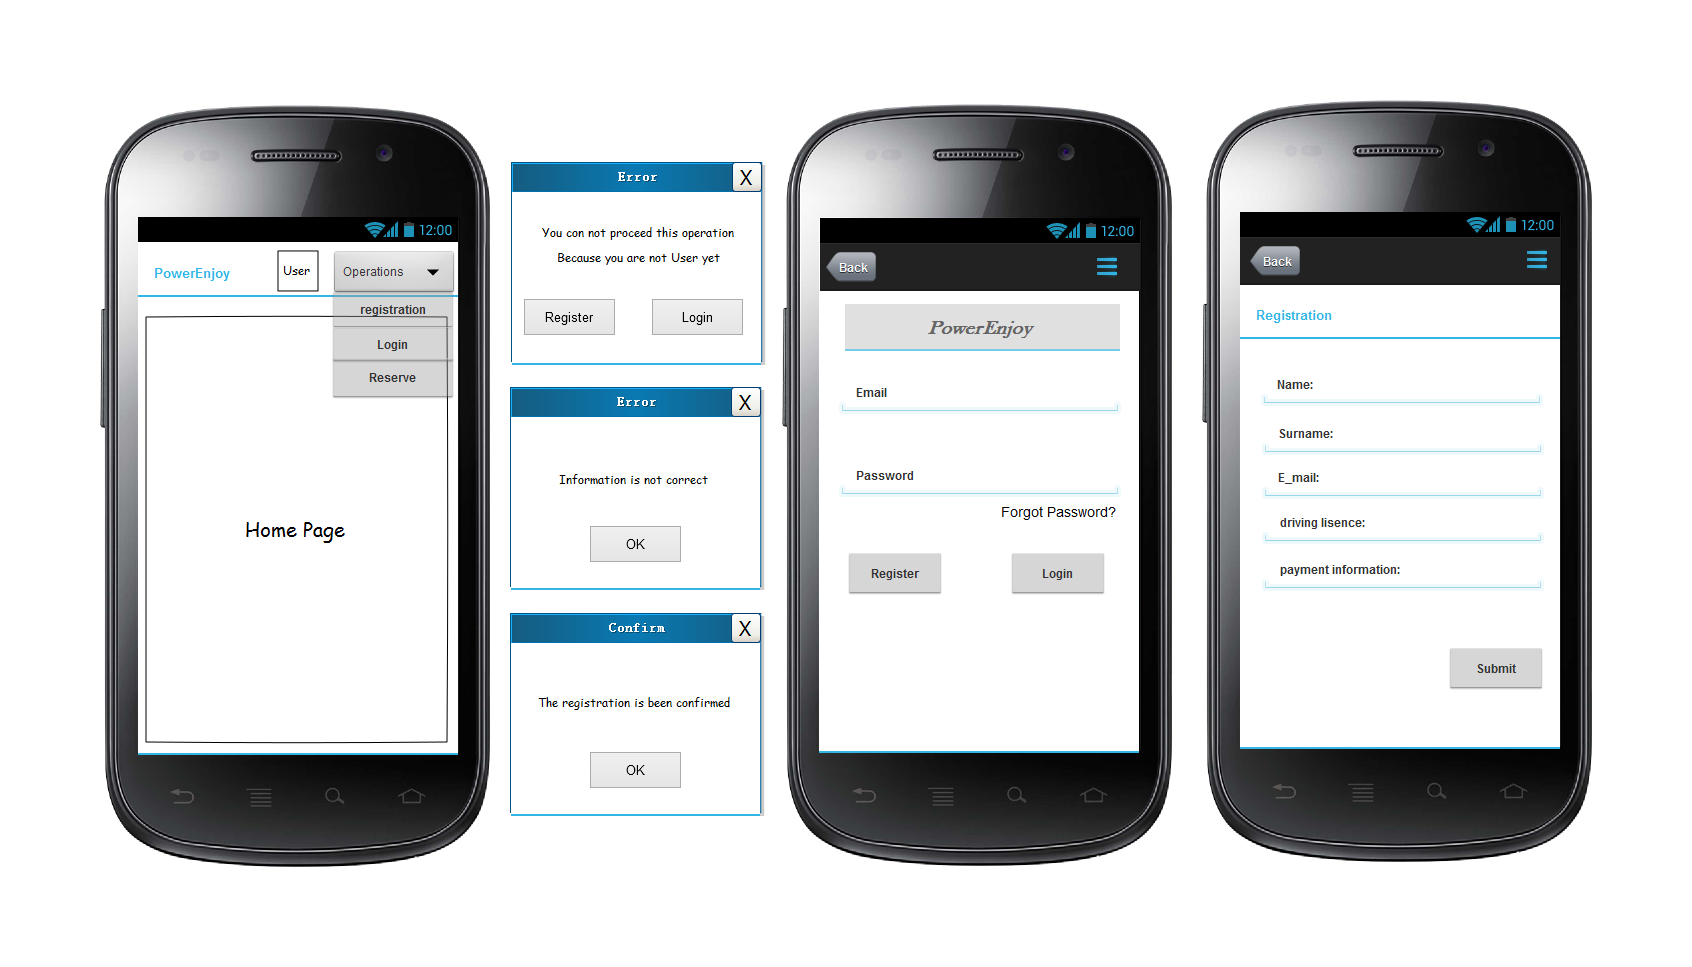
\includegraphics[width=\textwidth]{HomePage,Registration,Login} 
			\end{figure}
		In the HomePage(leftmost one) there are a menu list which contain the operation that user can do(registration, register,login).If a guest press the reservation, a window appear to notify guest to register or login. Other two interface are respectively Login and Register interface. After the submit, base on the result will open a pop-up window to notify user.
			\newpage
		\subsection{Registration,Pick up}
			\begin{figure}[h]
				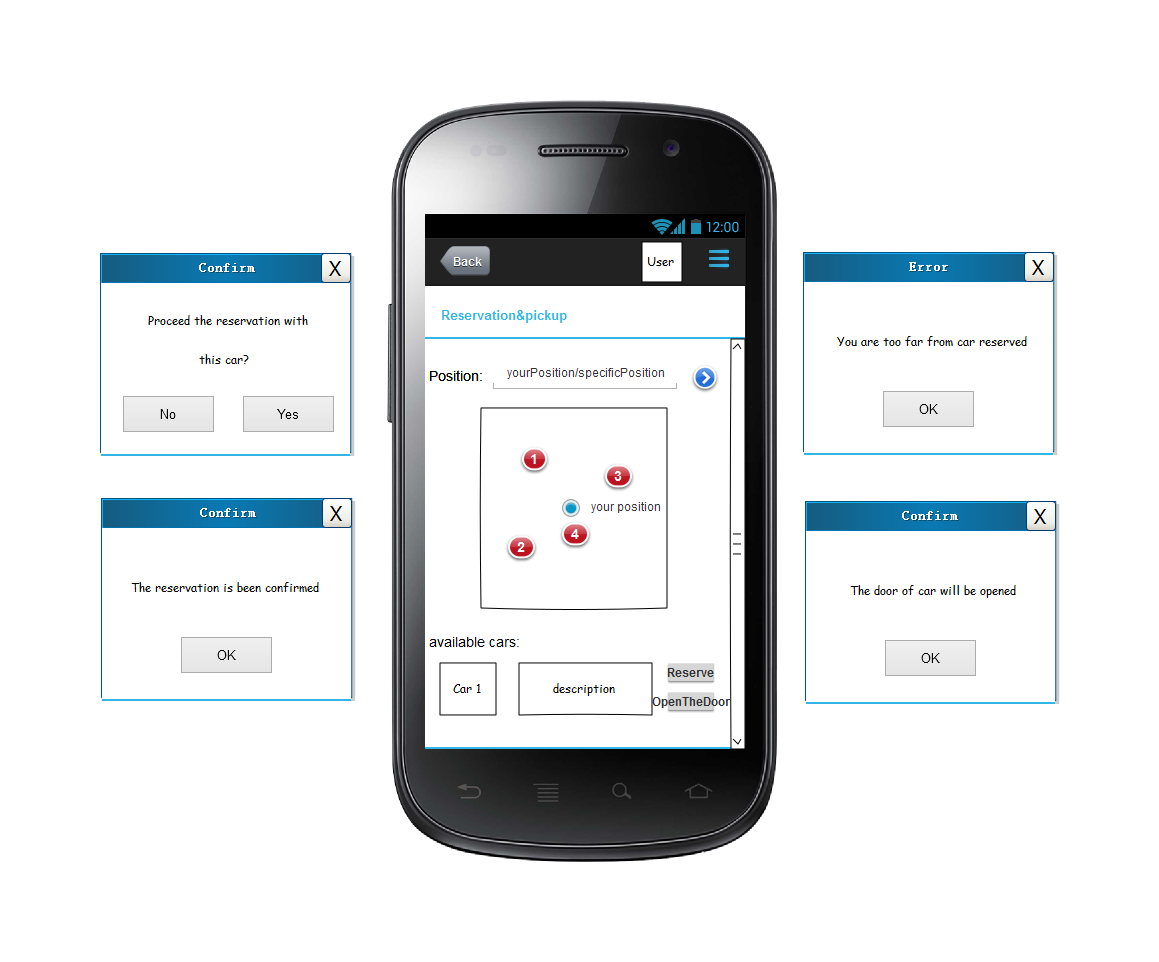
\includegraphics[width=\textwidth]{Reservation,PickUp} 
			\end{figure}
		In this page, user can indicate the position to start ride, and a map to show available car at that position. There is a button of reserve the car indicate, and other one to open the door of car(it can be pressed only you have already reserve corresponding car). There are also some pop-up window to indicate message for user. 
		\newpage
		\subsection{Screen on the car}
			\begin{figure}[h]
				\centering
				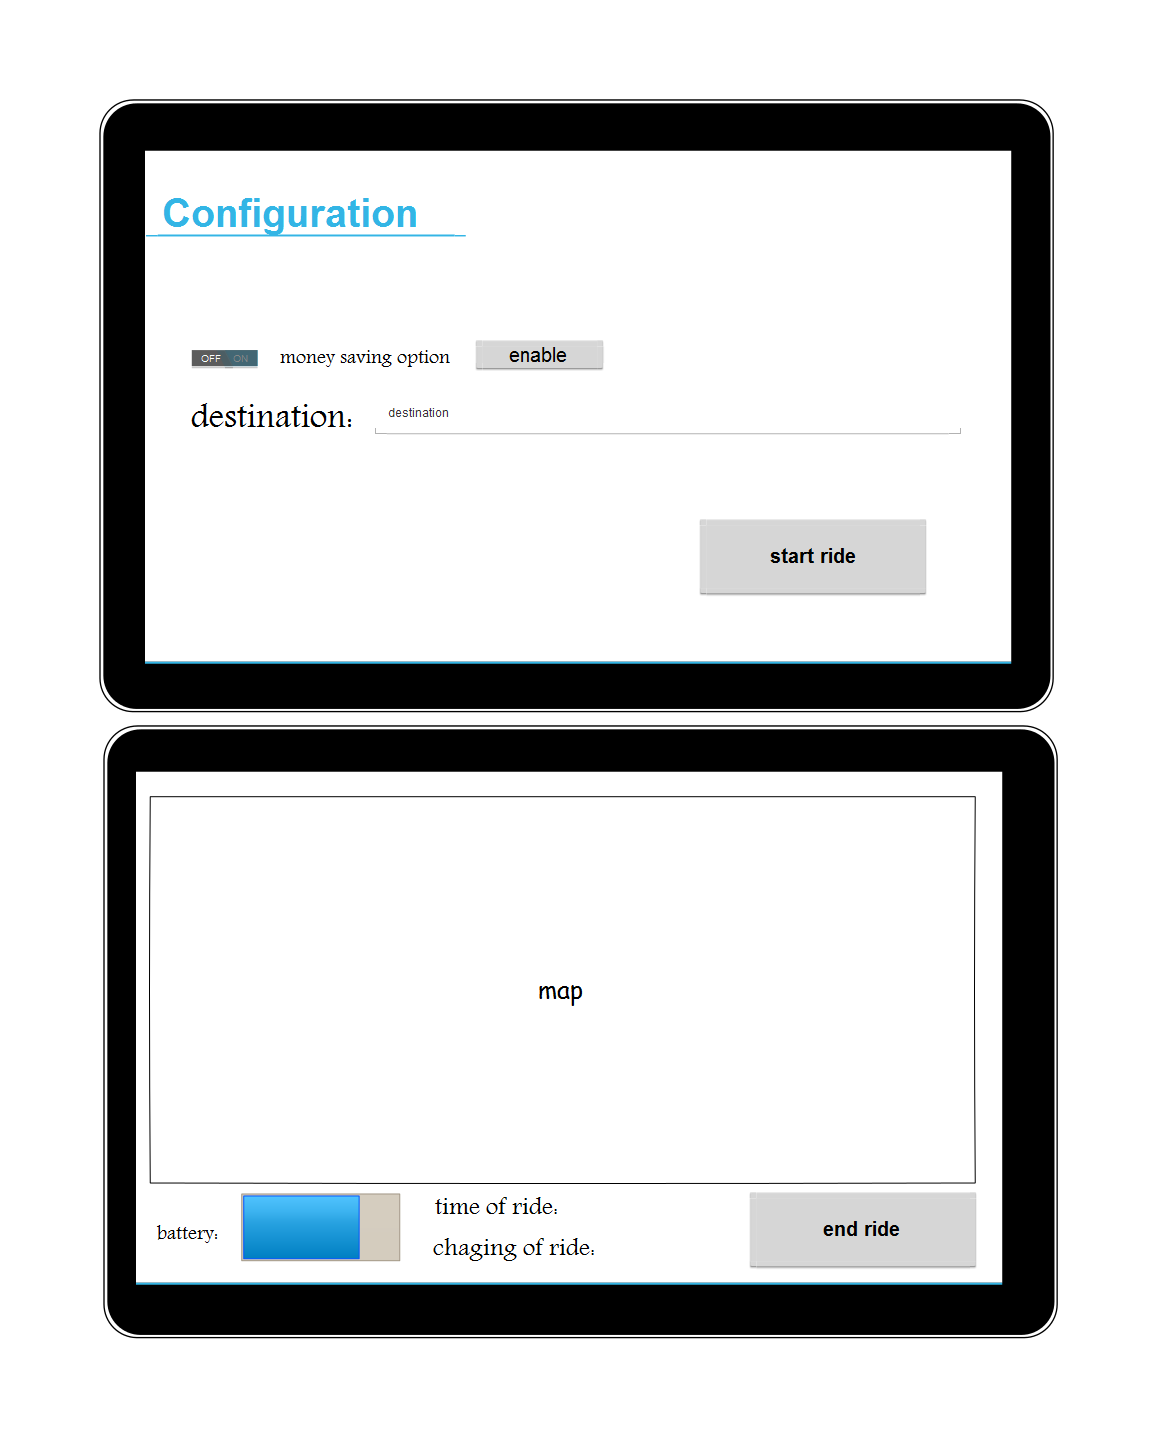
\includegraphics[scale=0.25]{Screen.png} 
			\end{figure}
			At initial page of screen, user can either to enable the money save option or not,if it's former case user will indicate destination, then use button START RIDE to ignite engine. Bottom one is the page during the ride to show to user for information related at ride.And END RIDE button to finish the ride. 
\end{document}